
\documentclass{article}

\usepackage{graphicx}
%\usepackage[backend=bibtex, style=verbose-trad2]{biblatex}
\usepackage{url}
\usepackage{hyperref}

\begin{document}
  \title{Hello World!}
  \date{}
\maketitle

%http://airesearch.com/ai-groups/how-alphago-mastered-the-game-of-go-with-deep-neural-networks/

\begin{figure}[h!]
  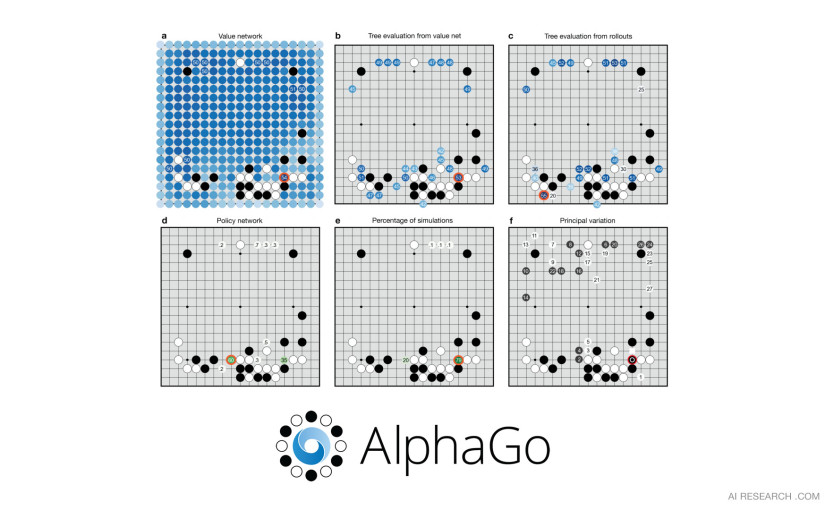
\includegraphics[width=\linewidth]{alpha_go.jpg}
 	For more info chek \cite{Alpha_GO}. 
  \label{fig:boat1}
\end{figure}

\newpage
{\small
\begin{thebibliography}{9999}

\bibitem{Alpha_GO} 
\textit{How AlphaGo Mastered the Game of Go with Deep Neural Networks},
 Artificial Intelligence, \textbf{1} (2016) \url {http://airesearch.com/ai-groups/how-alphago-mastered-the-game-of-go-with-deep-neural-networks/ } , by ai-research
\end{thebibliography}
}


\end{document}